\part{Version control: the basics}
\frame{\partpage}

\begin{frame}{What is version control?}
    \begin{itemize}
        \item A system for managing \textbf{changes} to source code
        \item Tracks the \textbf{history} of changes
        \item Allows changes from multiple developers to be \textbf{merged}
        \item Allows for multiple \textbf{forks} and \textbf{branches} of the same code
    \end{itemize}
\end{frame}

\begin{frame}{Why use version control?}
    Here's what \textbf{life without version control} looks like:
    \begin{itemize}
        \item You need to make \textbf{manual backups} of your code
        \item It's hard (or impossible) to \textbf{undo} a change
        \item Maintaining \textbf{multiple copies} of the codebase (e.g.\ production, development, testing)
            is a hassle
        \item Work from \textbf{multiple developers} needs to be manually copied and pasted together
        \item Code needs to be \textbf{transferred} around by dropbox / email / flash drive
    \end{itemize}
    Version control (used properly!) \textbf{takes care of all of the above}
\end{frame}

\begin{frame}{What is Git?}
    \begin{center}
        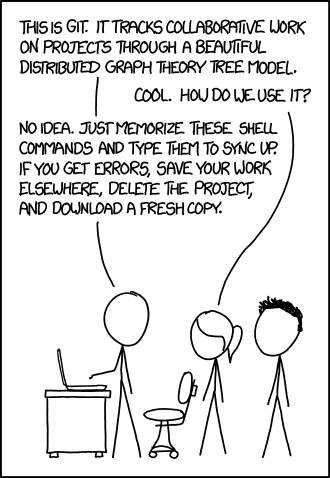
\includegraphics[height=0.7\textheight]{xkcd1597}
        
        {\tiny\url{https://xkcd.com/1597/}}
    \end{center}
\end{frame}

\begin{frame}{What is Git?}
    \begin{itemize}
        \item \textbf{Git} is an open-source \textbf{distributed version control system}
        \item Originally developed by Linus Torvalds and other Linux kernel developers
        \item \textbf{GitHub} is a site that provides free Git hosting
    \end{itemize}
\end{frame}

\begin{frame}{Basic Git workflow}
    \begin{itemize}
        \item \textbf{Origin repository}: the repository on GitHub's servers
        \item \textbf{Local repository}: a copy of the repository on your local machine
            (usually stored in a folder named \texttt{.git})
        \item \textbf{Working copy}: the source files you are editing
    \end{itemize}
\end{frame}

\begin{frame}{Basic Git workflow}
    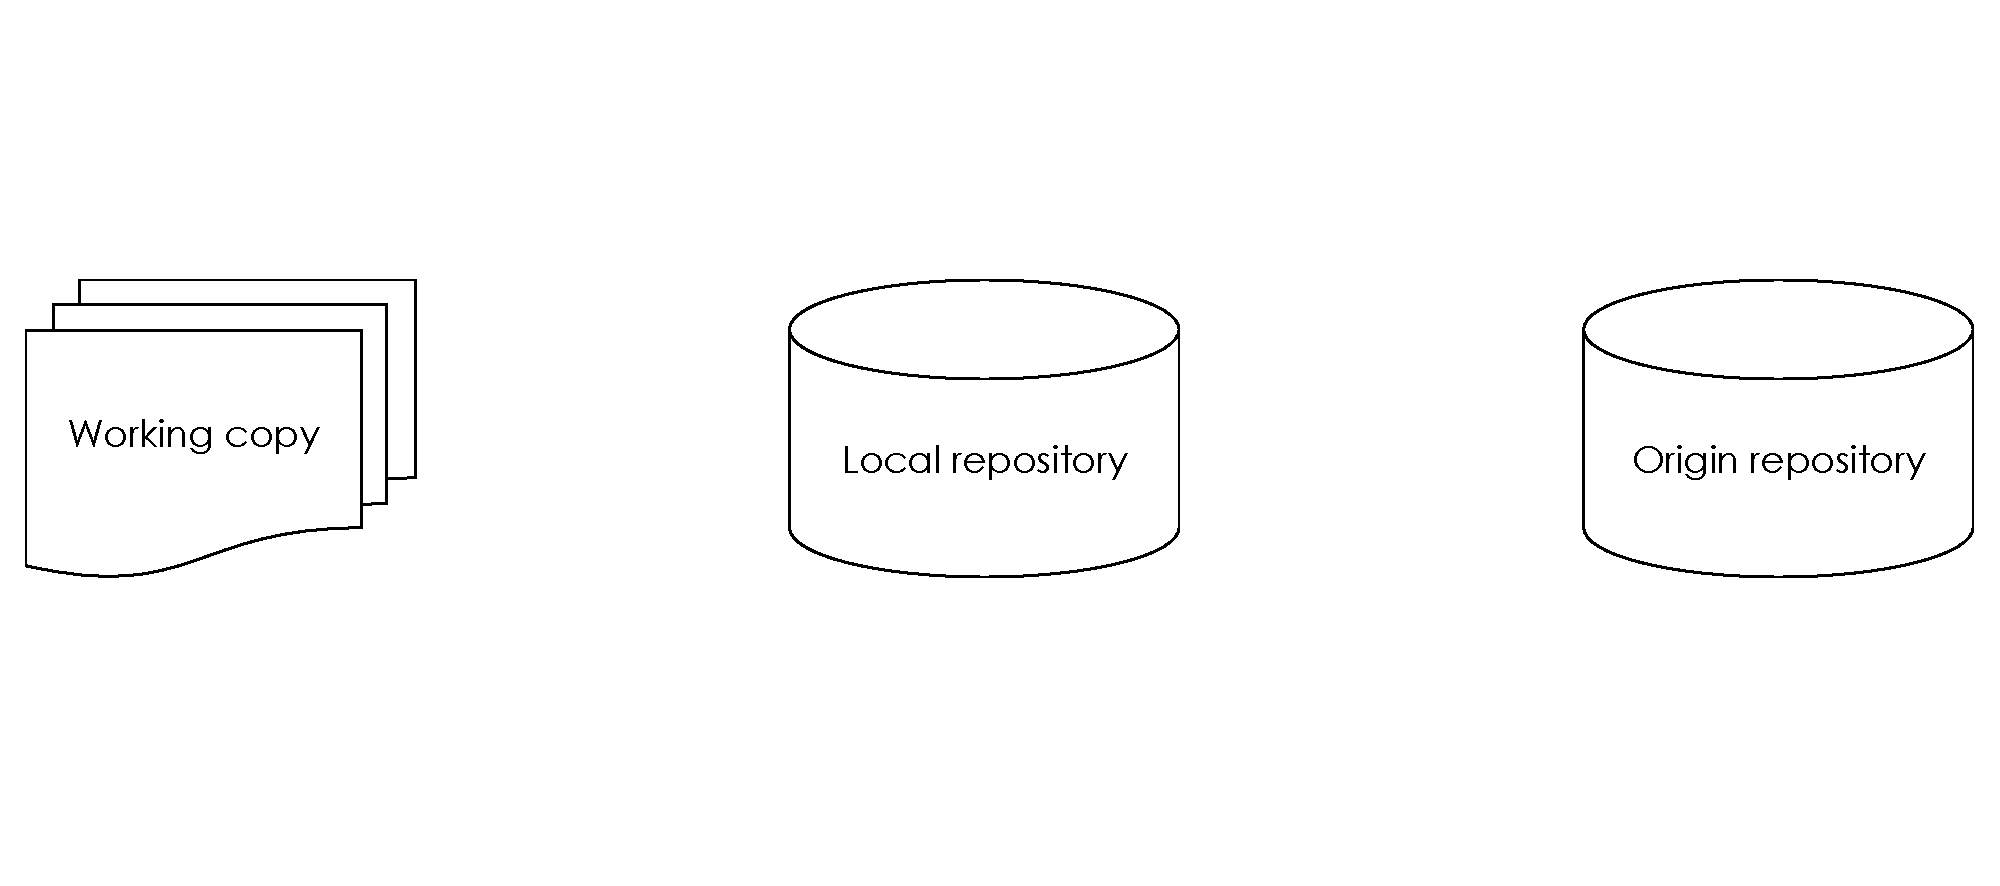
\includegraphics[width=\textwidth]{github_workflow_1}
\end{frame}

\begin{frame}{Basic Git workflow}
    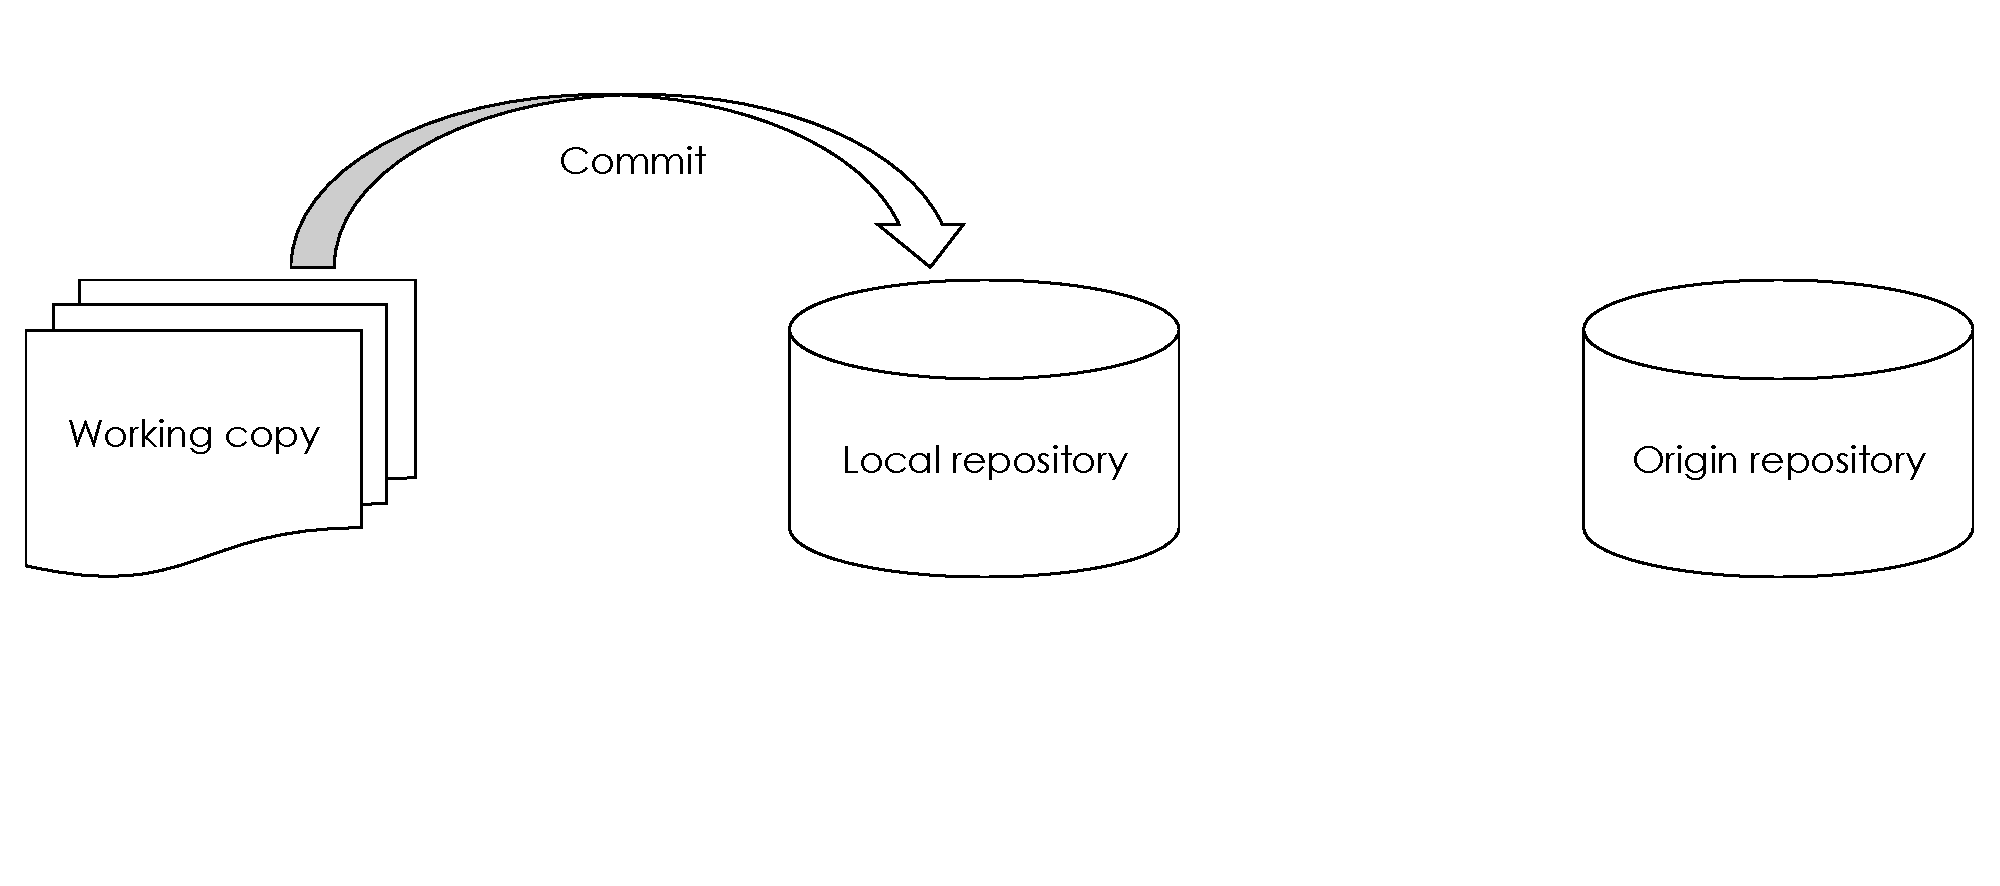
\includegraphics[width=\textwidth]{github_workflow_2}
    
    \textbf{Commit} adds your recent changes to your local repository
\end{frame}

\begin{frame}{Basic Git workflow}
    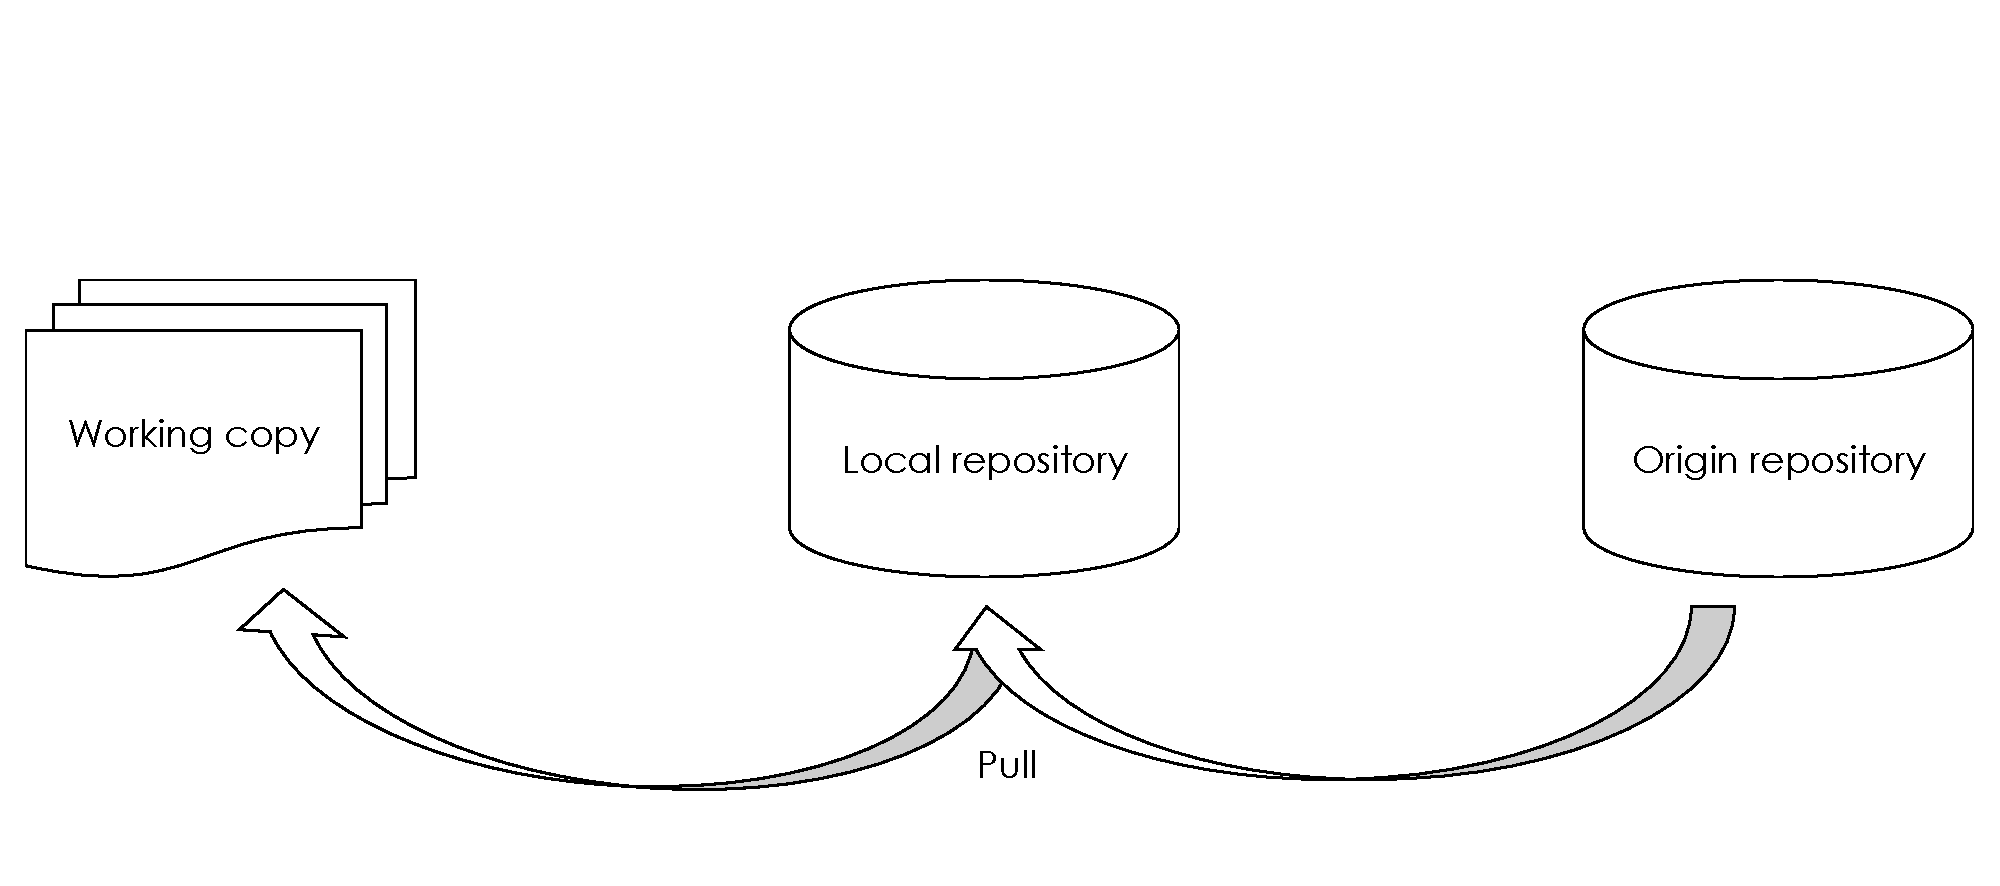
\includegraphics[width=\textwidth]{github_workflow_3}
    
    \textbf{Pull} fetches any changes from the GitHub server
\end{frame}

\begin{frame}{Basic Git workflow}
    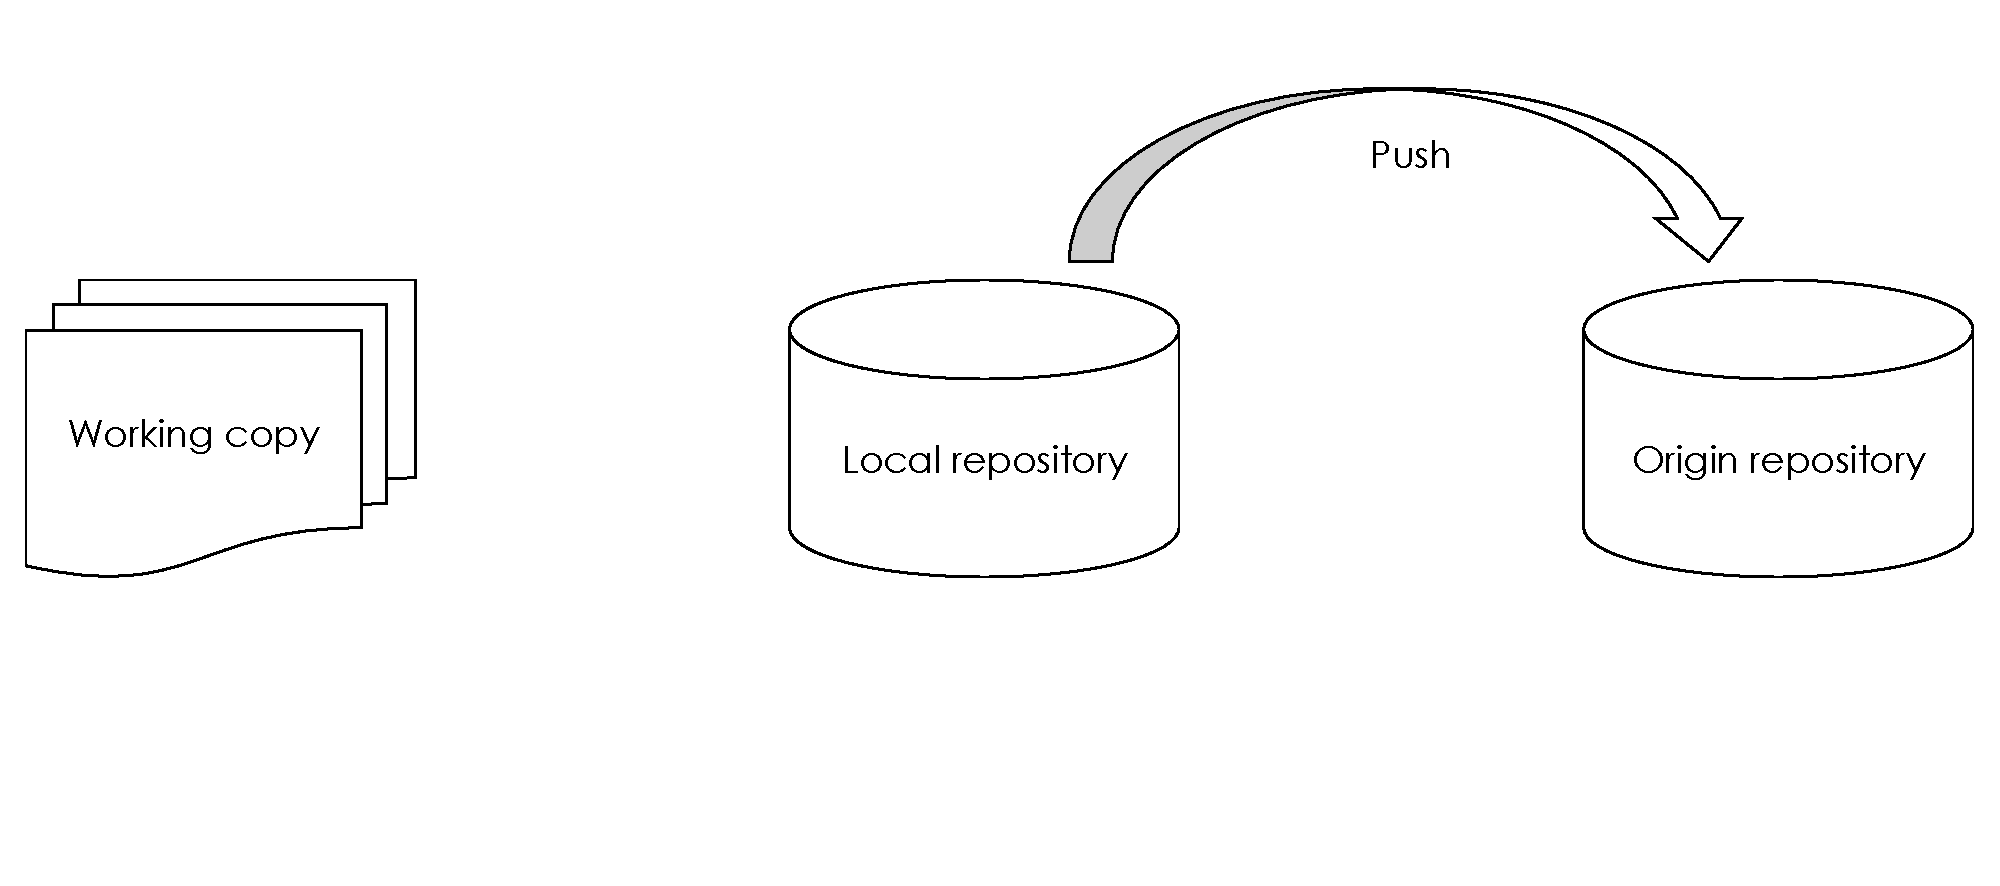
\includegraphics[width=\textwidth]{github_workflow_4}
    
    \textbf{Push} sends your committed changes to the GitHub server
\end{frame}

\begin{frame}{Basic Git workflow: recap}
    \begin{itemize}
        \item \textbf{Commit} when you have changed something
        \item \textbf{Pull} to fetch the latest changes from the server
        \item \textbf{Push} to upload your changes to the server
        \item Generally want to stick to doing things in this order, in particular:
            \begin{itemize}
                \item Always \textbf{pull} before you \textbf{push}
                \item Always \textbf{commit} before you \textbf{pull}
            \end{itemize}
        \item Some clients (e.g.\ GitHub for Windows)
            combine pull and push into a single \textbf{sync} command
    \end{itemize}
\end{frame}

\begin{frame}{When to commit}
    \begin{itemize}
        \item \textbf{Commit early and commit often}
        \item If you implement something, test it and it works, commit it!
        \item \textbf{Rule of thumb}: if it takes more than one sentence to describe what you have changed,
            you should have committed earlier!
    \end{itemize}
\end{frame}

\begin{frame}{Commits are changes}
    \begin{center}
        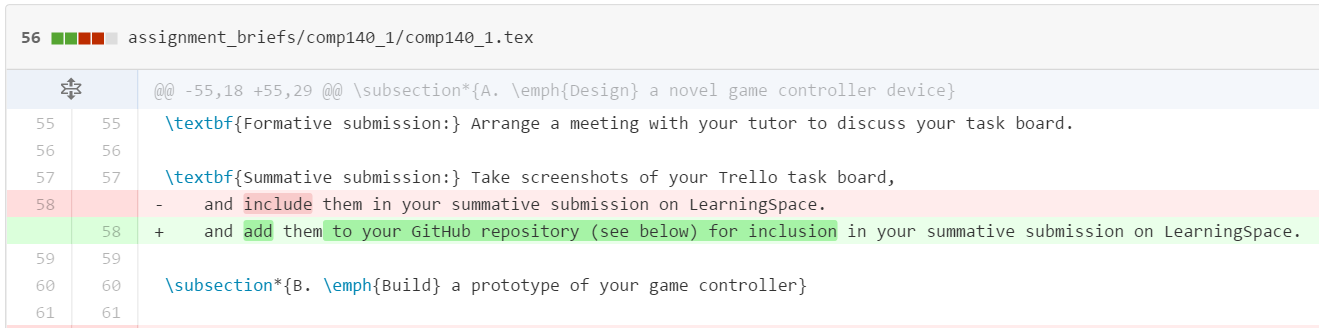
\includegraphics[width=\textwidth]{diff}
    \end{center}

    \begin{itemize}
        \item A commit is a set of \textbf{changes} to files
        \item A commit \textbf{is not} a snapshot of the code (although it can be used to make one)
    \end{itemize}
\end{frame}

\begin{frame}{Collaborative development}
    \begin{itemize}
        \item Alice changes something in \texttt{game.cpp}, commits it and pushes it
        \item \textbf{Meanwhile}, Bob changes something in \texttt{game.cpp} and commits it
        \item Bob pulls Alice's changes. What happens?
    \end{itemize}
\end{frame}

\begin{frame}{Merging changes}
    \begin{itemize}
        \item If Alice \textbf{hasn't} edited any of the \textbf{same lines of code} as Bob,
            Git will \textbf{merge} the changes automatically
            \begin{itemize}
                \item NB: Git is clever about figuring out \textbf{where} a change should be applied ---
                    e.g.\ it \textbf{doesn't} just use line numbers,
                    so inserting code earlier in the file shouldn't mess it up
                \item Bob will see \textbf{both} his and Alice's changes, and so will Alice next time she pulls
            \end{itemize}
        \item If they \textbf{have} edited the same lines, Git won't be able to merge them automatically
            --- this is a \textbf{conflict!}
    \end{itemize}
\end{frame}

\begin{frame}[fragile]{Resolving conflicts}
    \begin{itemize}
        \item If there is a conflict, the offending file will look like this:
    \end{itemize}
    \begin{lstlisting}
int main(int argc, char* argv[])
{
    std::cout << "Hello world!" << std::endl;
<<<<<<< HEAD
    std::cout << "My name is Bob!" << std::endl;
=======
    std::cout << "My name is Alice!" << std::endl;
>>>>>>> origin/master
    return 0;
}
    \end{lstlisting}
    \begin{itemize}
        \item You are given \textbf{both versions} of the code ---
            you need to \textbf{manually edit} the code to make sense again
    \end{itemize}
\end{frame}

\begin{frame}[fragile]{Resolving conflicts}
    \begin{lstlisting}
int main(int argc, char* argv[])
{
    std::cout << "Hello world!" << std::endl;
    std::cout << "Our names are Alice and Bob!" << std::endl;
    return 0;
}
    \end{lstlisting}
    \begin{itemize}
        \item After editing \textbf{and testing}, commit and push as normal
    \end{itemize}
\end{frame}

\begin{frame}[fragile]{Prevention is better than the cure}
    \begin{itemize}
        \item In a properly managed project, conflicts should be a \textbf{rarity}
        \item \textbf{Coordinate} your efforts so that developers are not working on the same lines of code
            at the same time
        \item Use a sensible \textbf{branching} strategy (see later) to manage and plan the times when
            code is to be merged
    \end{itemize}
\end{frame}

